\documentclass[12pt,a4paper]{article}
%%%! Tjulin: I would use \documentclass[12pt,a4paper]{article} for the benefit of European printers 
%% JW: DONE

% \usepackage{array}
% \usepackage{pbox}
% \usepackage{hanging}
\usepackage{fancyhdr}
% \usepackage{caption}
% \usepackage{enumitem}
\usepackage{fancyvrb}
\usepackage{color}
\usepackage[utf8]{inputenc}
\usepackage{graphicx}
\usepackage{listings}
\usepackage{url}
\usepackage[titletoc,title]{appendix} %%%! Tjulin: Added this for the appendices. 
%% JW Thanks.

\usepackage{xspace}

\usepackage{rotating}
\usepackage{wrapfig}
\usepackage{hyperref}

\usepackage{cite} %

\usepackage[gen]{eurosym}

% \usepackage{draftwatermark}
% \SetWatermarkText{draft v2}
% \SetWatermarkScale{6}

\fancypagestyle{plain}{ %
  \fancyhf{} % remove everything
  \renewcommand{\headrulewidth}{0pt} % remove lines as well
  \renewcommand{\footrulewidth}{0pt}
}

\hyphenation{EISCAT}

\newenvironment{MYitemize}{%
    %% \renewcommand{\labelitemi}{$\rightarrow$}%
    %% \renewcommand{\labelitemii}{$\circ$}%
    %% \renewcommand{\labelitemii}{$\rightarrow$}%
    %% \renewcommand{\labelitemiii}{$\rightarrow$}%
    %% \renewcommand{\labelitemiii}{\colblack $\cdot$}%
    \begin{itemize}}{\end{itemize}}

\newcommand{\bitm}{\begin{MYitemize}}
\newcommand{\eitm}{\end{MYitemize}}

\newcommand{\ED}{EISCAT\_3D\xspace}
\newcommand{\EC}{EISCAT\xspace}
\newcommand{\ESA}{EISCAT Scientific Association\xspace}
\newcommand{\SA}{sub-array\xspace}
\newcommand{\SAs}{sub-arrays\xspace}
\newcommand{\RS}{radar site\xspace}
\newcommand{\RSs}{radar sites\xspace}
\newcommand{\OS}{on-site\xspace}
\newcommand{\OC}{operations centre\xspace}
\newcommand{\CC}{control centre\xspace}
\newcommand{\DC}{data centre\xspace}
\newcommand{\DCs}{data centres\xspace}
\newcommand{\UAF}{User Analysis Facility\xspace}

\newcommand{\RB}{ring buffer\xspace}
\newcommand{\fsru}{first stage receive unit\xspace}
\newcommand{\FW}{file writer\xspace}
\newcommand{\SBF}{second beam former\xspace}

\newcommand{\NBW}{5~MHz} % narrow bandwidth
\newcommand{\WBW}{30~MHz} % wide bandwidth

\newcommand{\ramf}{Ramfjordmoen\xspace}
\newcommand{\controllatency}{less than $5$\xspace}
\newcommand{\HDF}{HDF5\xspace}
\newcommand{\einfra}{e-infrastructure\xspace}
\newcommand{\einfras}{\einfra{s}\xspace}
\newcommand{\WR}{White Rabbit\xspace}
\newcommand{\UAP}{User access portal\xspace}

\newcommand{\bfmust}{\xspace{\bf must}\xspace}
\newcommand{\bfshould}{\xspace{\bf should}\xspace}
\newcommand{\Bfmust}{\xspace{\bf Must}\xspace}
\newcommand{\Bfshould}{\xspace{\bf Should}\xspace}
\newcommand{\bfshall}{\xspace{\bf shall}\xspace}
\newcommand{\Bfshall}{\xspace{\bf Shall}\xspace}

\newcommand{\FirstBF}{\xspace{\bf Shall}\xspace}

\newcommand{\visroot}{isualiz}
\newcommand{\vis}{\visroot{ation}\xspace}
\newcommand{\vise}{\visroot{e}\xspace}
% \newcommand{\Vis}{{Visualization}\xspace}
\newcommand{\threed}{{3-dimensional}\xspace}
\newcommand{\GD}{{GUISDAP}\xspace}

\newcommand{\gps}{{Gbit/s}\xspace}


\newcommand\EatDot[1]{}



% \setlength{\topskip}{0mm}
\setlength{\headheight}{15pt}
% \setlength{\topmargin}{-5.4mm}
% \setlength{\textheight}{230mm}
\setlength{\textwidth}{180mm}
\setlength{\oddsidemargin}{-5.0mm}
% \setlength{\evensidemargin}{10.0mm}
% \setlength{\captionmargin}{7mm}

\title{
{\bf Deliverable Document 1} \\
On-site computing software and hardware architecture
recommendation}
\author{E3DDS Team~\footnote{
Anders Tjulin (EISCAT) {\tt anders.tjulin@eiscat.se};
Ari Lukkarinen (CSC) {\tt ari.lukkarinen@csc.fi};
Assar Westman (EISCAT) {\tt Assar.Westman@eiscat.se};
Carl-Fredrik Enell (EISCAT) {\tt carl-fredrik.enell@eiscat.se};
Dan Johan Jonsson (UiT) {\tt dan.jonsson@uit.no};
Janos Nagy (NSC) {\tt fconagy@nsc.liu.se};
Harri Hellgren (EISCAT) {\tt harri@eiscat.se};
Ingemar H\"{a}ggstr\"{o}m (EISCAT) {\tt ingemar.haggstrom@eiscat.se};
Mattias Wadenstein (UmU) {\tt maswan@hpc2n.umu.se};
Roy Dragseth (UiT) {\tt roy.dragseth@uit.no};
John White (NeIC) {\tt john.white@cern.ch}}}

\date{\today}

\begin{document}

\pagestyle{fancy}
\lhead{\bf E3DDS project}
\rhead{\bf 1: Hardware and software}

\maketitle
\par\noindent
\begin{minipage}{0.45\textwidth}
  
\includegraphics[scale=0.18]{NEIC_logo_screen_black.pdf}
  %\vspace{-0.09in}
\end{minipage}
\begin{minipage}{0.45\textwidth}
  \hfill
  %
\includegraphics[scale=0.25]{EISCAT3Dlogo1.pdf}
  % New official logo with green text
  
\includegraphics[width=0.75\linewidth]{e3d-logo-green-500px}
\end{minipage}

\begin{center}
\begin{tabular}{|l|l|} \hline
\large \bf Date & \large \bf Comments \\ \hline
\large 2018/06/19 & First draft started \\ \hline
\large 2018/12/07 & Reviewed by Anders \\ \hline
\large 2018/12/17 & Sent to SG \\ \hline
\large 2019/01/23 & Accepted by SG \\ \hline
\large 2019/08/07 & Added hyperref package to fix links\\ \hline

% \large \today  & Current \\ \hline
\end{tabular}
\end{center}

\newpage
\tableofcontents
\newpage

%%%! Tjulin: It would be nice with an "Executive Summary" or "Abstract" for the lazy reader

\section{Executive Summary}
\label{exec-summ}

The on-site computing, network and storage needs for the \ED transmitting and receiving sites have been discussed and calculated to not vary much from initial estimates.

%%% C-F Enell: The following sentences are awkward. 
% The choice of the input network from the First Stage Receiving Units to the second beam former servers alternates between a direct connection %to the FSRU to servers or a switching network.
There are two possible choices of input network architecture between the First Stage Receiving Units to the second beam former: a switch fabric or direct connections from FSRUs to second beamformer servers. A comparative pricing for each option is included.
Discussions including networking experts and FSRU manufacturer have concluded that the optimal output connections are $2 \times 25$~Gb/s optical. 

The second beam former is presently calculated to require 40 2U server nodes for real-time FIR filtering at \NBW\ bandwidth rates.
The FIR filter outputs must also be summed in realtime at \NBW\ bandwidth.
Either more 2U server nodes need to be added to accommodate the summation or a high-performance switching fabric downstream of the server nodes will perform the summations.

The processes that write the summed second beam former results to files are proposed to run on the \SBF\ servers OR on dedicated servers downstream but before the site-local buffer.

The optimum configuration for the site-local buffer is proposed to be RAID-5 SSDs directly integrated to the second beam former nodes.
This is instead of the first-proposed separate disk array.

\section{Purpose}
\label{purpose}
%%%! Tjulin: This little section looks more like "Planned work to do" than "Purpose of the document and work done". Could be rewritten somewhat.
%% JW re-written
This document describes and recommends the on-site computing software and hardware architectures for \ED. 
These recommendations are the outcome of iterative discussions between the \ED software engineers and scientists and national provider deployment experts. 
The architecture is a result of close discussions and work between the on-site computing (beam former, Level 2 data processing, Level 3 data analysis and possibly satellite screening code) developers, EISCAT scientists and the operators of the national \einfras.
This document describes the prototype software to be written and gives the software and hardware recommendations.

%%%! Tjulin: Who is the target reader of the report? 
%% JW Added.
The target readers of this document are primarily the \ED project management and scientists.
The \ED project management can get an indication of the actual amount of computing at the different \ED sites.
Also, another target is the providers of the national \einfras where \ED will be located.
The national \einfra providers can see the quantity and type of computing required for \ED and make determinations whether some can be run in existing computing centres.

\section{Introduction}
\label{intro}

The \ESA will establish \ED, a flexible multistatic high power radar system, that
will enable comprehensive three-dimensional vector observations of the atmosphere
and ionosphere above Northern Fenno-Scandinavia.  

The use of new radar technology, combined with the latest advances within digital signal processing,
will achieve ten times higher temporal and spatial resolution than
obtained by the present \EC radar systems. For the first time, \EC will also be able to measure continuously.  
The flexibility of the \ED system will enable scientists to investigate upper-atmospheric and 
ionospheric phenomena at both large and small scales unobtainable by the present systems.

In its first stage, the \ED system will consist of three \RSs:
one having both {\bf T}ransmitting ({\bf TX}) and {\bf R}eceiving ({\bf RX})
capabilities and two with only RX capability.  
The sites will
be remote-controlled and located in three different countries (Finland,
Norway and Sweden) and will be separated geographically by
approximately 130~km.  
Two additional receiver sites, at distances 200-250~km from the transmit site, 
are planned for the full \ED system at a later stage.

\ED will produce data at three levels, from raw samples to physical parameters. Table~\ref{tab:datalevels} summarizes the \ED data levels.
% \begin{center}
\begin{table}[h]
% \begin{center}
\centering
\begin{tabular}{l|l l l c}
{Level} & {Type}        & {Produced by} &  {Storage } & {Format} \\ \hline
% \bf 0  & Sampled antenna        & Antenna & None & Binary \\
%        & voltages               & sub-arrays & & \\
\bf 1a & Ring buffer data                & $1^{\rm st}$ stage beam & 4 months$^*$ & UDP stream/ \\
       &                                 & former &  & HDF5  \\
\bf 1b & Beam-formed data                & $2^{\rm nd}$ stage beam & 4 months$^*$ & HDF5 \\
       &                                 & former & &  \\
\bf 2  & Time integrated                 & All sites & Archived & \HDF \\
       & correlated data & & & \\
\bf 3a & Physical parameters             & All sites & Archived & \HDF \\
\bf 3b & 3D-voxel parameters             & Operations centre & Archived & \HDF \\
\bf 4  & Derived geophysical & Users & Users & Publications etc \\
       & parameters & & & 
\end{tabular}
\caption{Summary of the \ED data levels. 
The \ED \DCs will receive, serve and archive all data at levels 2 and 3.
{Data used in research should be given Persistent Identifiers (PIDs) according to a common standard such as DOI, DataCite, or similar, to be unambiguously citable in publications.}
(*)~A 4~months period is selected as this is the estimated time required
to perform a ``real-time'' analysis on low-level data.
A portion of the 
level~1 data will also be archived permanently, on the order of $1\%$
of the level~1 data rate, e.g. one beam per site and/or bandwidth-limited
data.
\label{tab:datalevels}}
% \end{center}
\end{table}
% \end{center}

This data will be curated, archived and catalogued.
This encompasses the management of the data throughout
its lifecycle, from initial storage to the time when it is moved to
long-term preservation for posterity or becomes obsolete and is
deleted. Metadata will be produced according to standardized metadata models and transferred to search portals. 

Also, for scientific publications using \ED data, a system to cite the data sets used should be provided in compliance with recommendations from funding agencies and the EU (FAIR principles are gaining importance: Findable, Accessible, Interoperable, Reusable). %%%! Tjulin: Is this a recommendation or a fact? 
Scientific work using and visualizing \ED data, or deriving other physical parameters by combining \ED data with other data, represents a fourth level. Derived data products produced by \ED users are indicated as Level~4 in the table, in addition to the three data levels produced by \ED.

%% CFE: use reference(s) to Fig 1
The \fsru attached to each \SA (Fig.~\ref{fig:central}) produces voltage-domain data from 10 
wide-angle beams  
as a series of data (level~1a) as a UDP bit-stream.
These data are buffered on the site RAM ring buffer and may be buffered for
4~months on the \OC storage.  
Likewise, the narrow angle beam files
(level~1b) from the second beam former are buffered for 4~months
on the \OC storage.  
A fraction (dependent on the experiment being
performed) of the first and second stage beam formed data will be
stored as persistent level~1 data files and sent to the \DCs.

%%%! Tjulin: Do we need to explain the E3D setup?  The data levels are defined but not "first stage" "sub-array" and so on.
%% Check with CF and Ingemar... I 

From the level~1b data, it will be possible to generate
\emph{lag profiles} (level~2 data), i.e. transform the data to the autocorrelation function domain. This is equivalent to power spectra, and thus the volume of level~2 data can be reduced by time averaging.
Physical parameters (level~3a data) will also be extracted by means of an inverse incoherent scatter model. 
The level~2 and~3a data from the three sites will be combined to produce level~3b data products: three-dimensional volume renderings of both scalar parameters and velocity vectors.

% All the data of levels~2 and~3 are to be archived at the \DCs.
The data will be buffered at the sites or / and a central storage 
and then transferred to the \DCs for long-term storage and access.
The previsioned container format of the data received at the \DCs from the \OC is \HDF~\cite{hdf}
(a standard data container library available for all considered programming languages). \HDF~based file formats are used by other radar systems such as AMISR~\footnote{Craig Heinselman, internal communication} and Millstone Hill (\url{https://github.com/MITHaystack/digital_rf}).

%%%! Tjulin: The "or / and" looks a bit odd in a document meant to provide recommendations on these issues.
%% CFE: not really since this deliverable concerns beamforming. Networking is a separate issue although addressed by NeIC (???)

\section{On-site hardware}
\label{sec-onsite-hw}

Figure~\ref{fig:central} gives the schematic representation of the data flow within a RX (or receiving on the TX) site from the antenna sub-array first beam former to the local site storage.
\begin{figure}
\centering
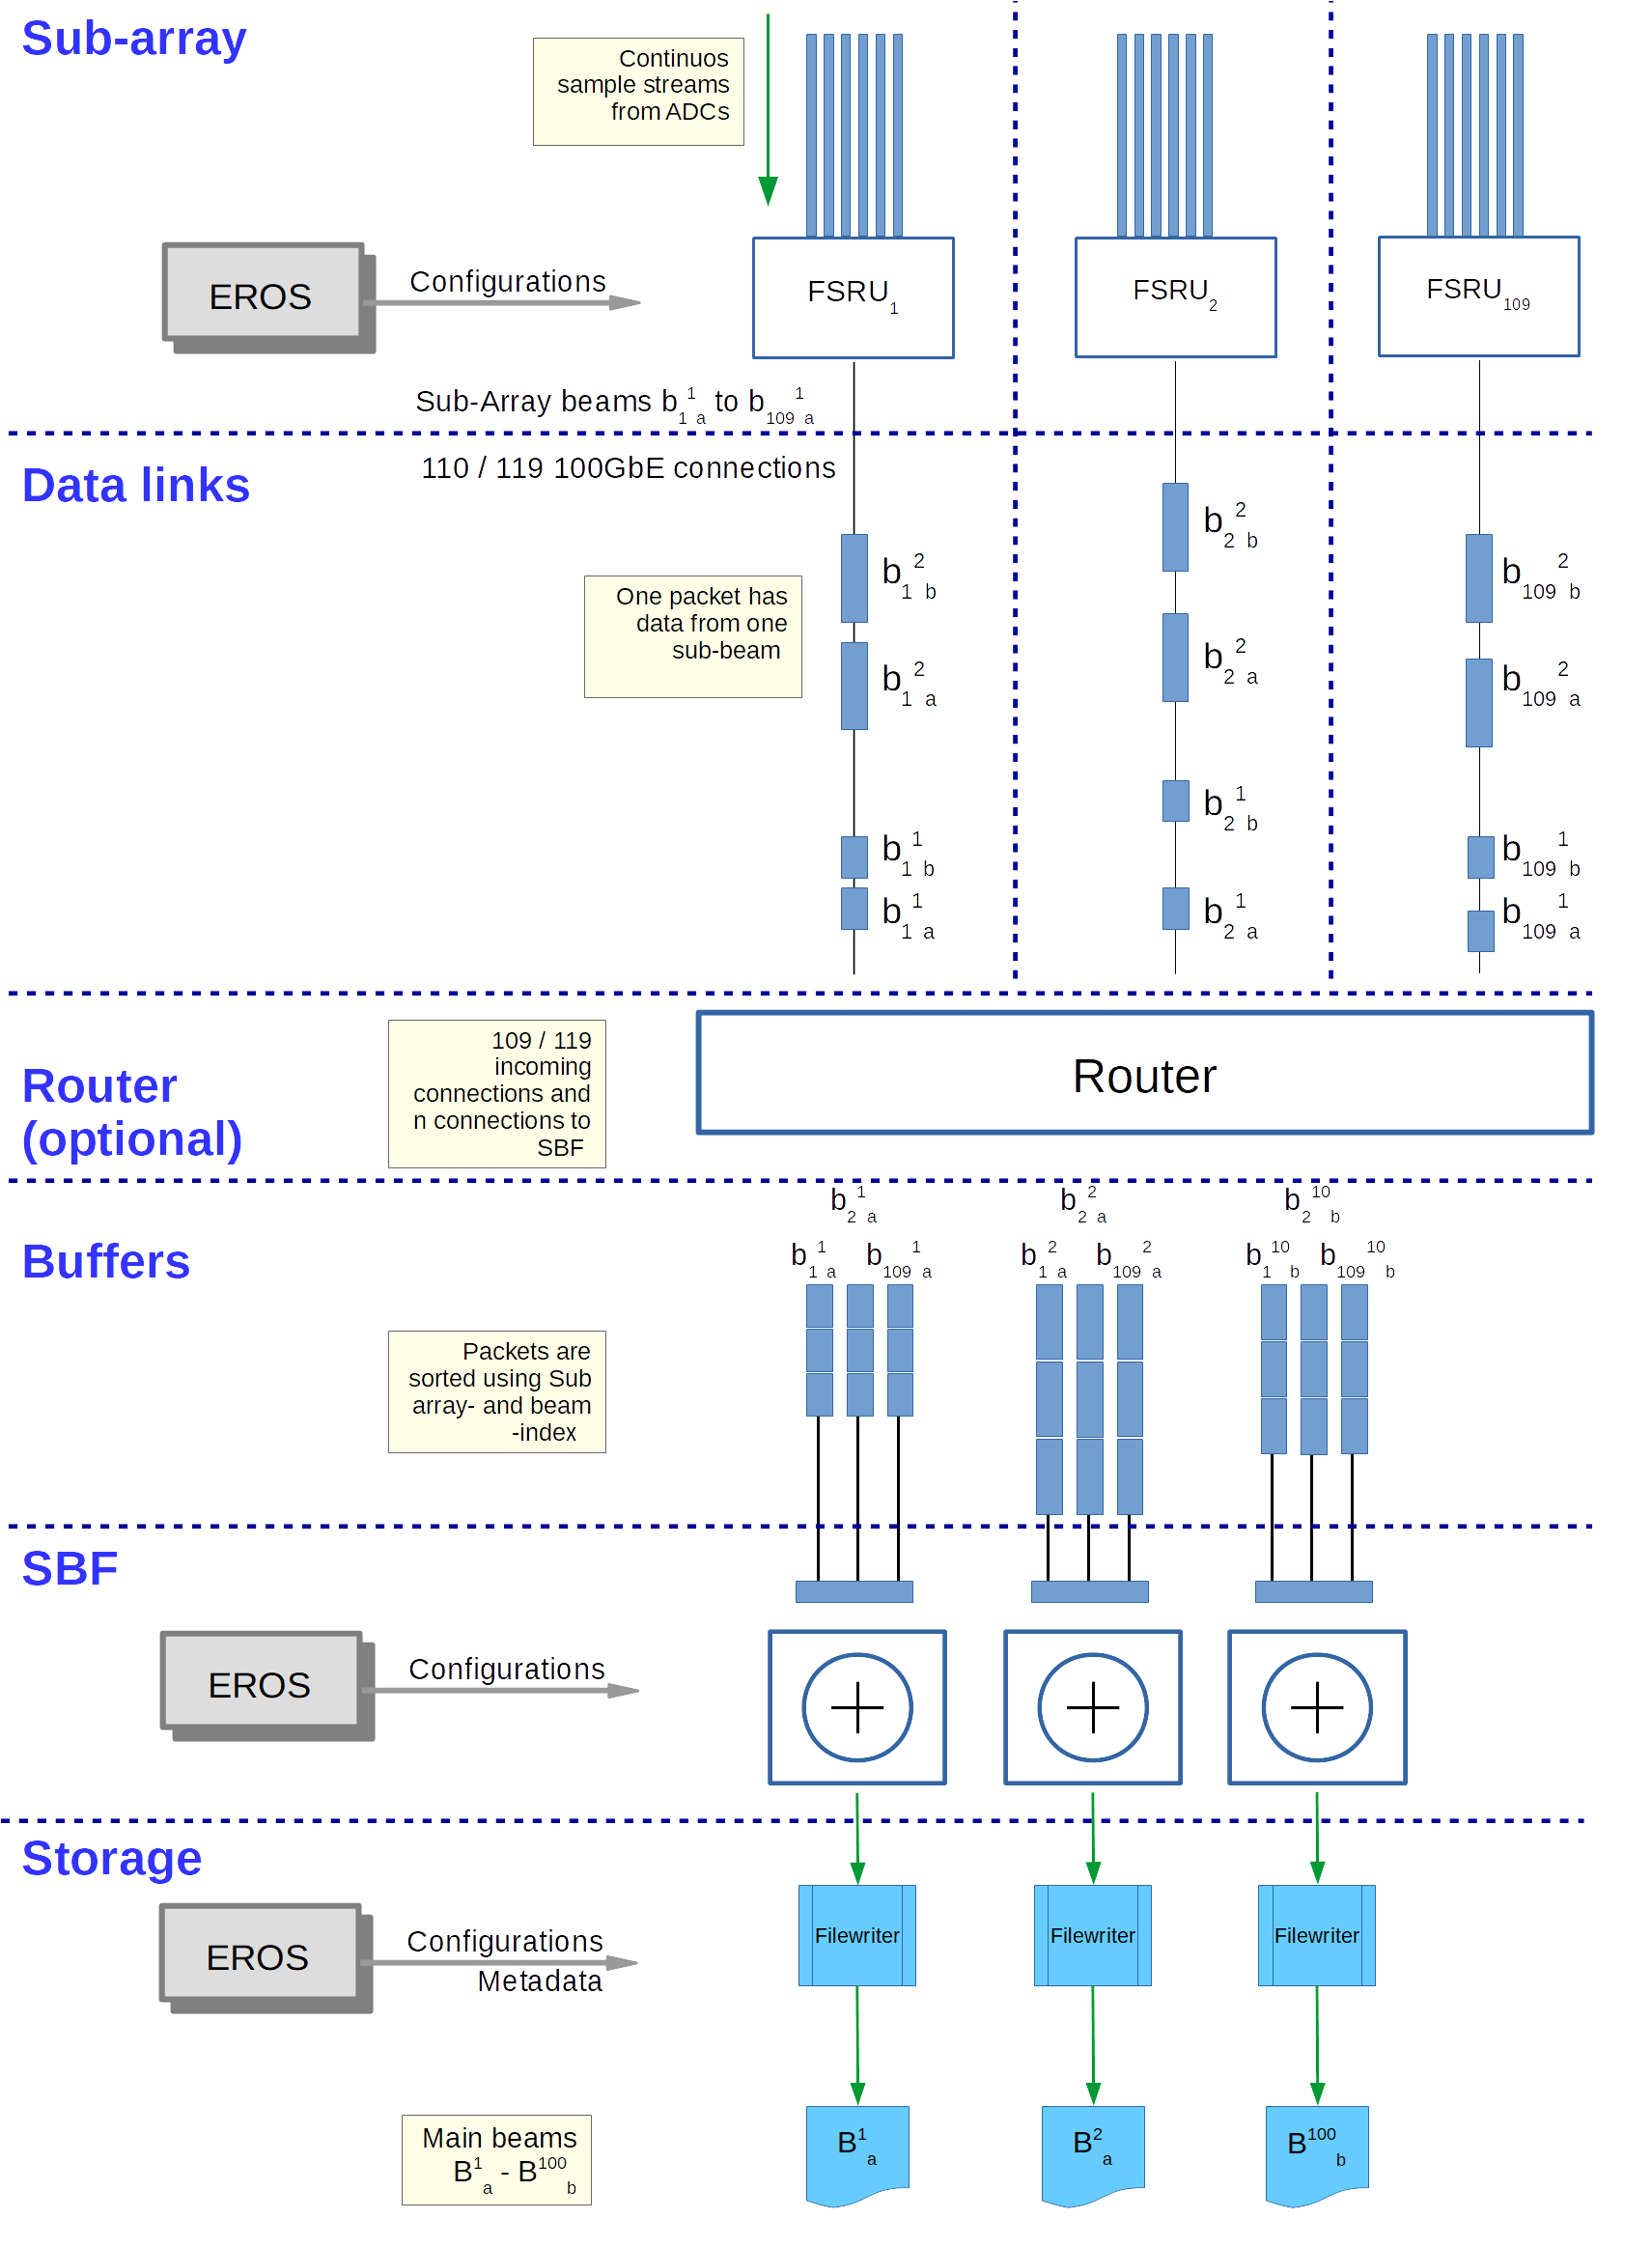
\includegraphics[width=0.7\textwidth]{E3D_dataflow_1aa.png}
\caption{Schematic of the on-site data flow from the sub-arrays to site storage.
\label{fig:central}
}
\end{figure}

The {\bf F}irst {\bf S}tage {\bf R}eceiving {\bf U}nit (FSRU) (FSRU$_s$ where $s=1,109~\footnote{There are 109 sub-arrays on the RX sites and 119 sub-arrays on the TX site.}$) attached to each of the site sub-arrays are shown at the top of Figure~\ref{fig:central}. 
Each FSRU outputs 10~wide-angle beams that are transmitted as UDP data packets 
(b${_s} {^n} {_p}$) where $s=1,109$ is the sub-array number, $n=1,10$ is the wide-angle beam number and  $p=a,b$ is the polarization of the beam.
The FSRUs are either directly connected to the computing nodes that contain the RAM \RB{}, or there is a switch that directs the UDP packets to the appropriate nodes.
The packets are written to the \RB ordered by beam number and polarization with all sub-array packets as a sequence
\{b${_1} {^1} {_a}$ ,... , b${_{109}} {^1} {_a}$\},
\{b${_1} {^1} {_b}$ ,... , b${_{109}} {^1} {_b}$\},
\{b${_1} {^2} {_a}$ ,... , b${_{109}} {^2} {_a}$\},\,\ldots{}\,, etc of $2180\,(109 \times 10 \times 2)$  wide-angle beams.

Each second beam former FIR filtering operations handles one beam from each sub-array for a total of 21800 filtering operations.
The outputs of the filter operations are summed to produce up to 200 narrow-angle ($0.6^{\circ}$ wide) beams~\footnote{The full \ED design specification will produce 100~narrow angle beams per polarization for a total of 200.}  (B${^m}{_p}$ where $m=1,10$ and $p=a,b$) 
% Are we sure this is an UDP stream, for the high-bandwidth case we talked earlier about
% these being transferred as MPI collective operations or other approaches?
transmitted to file writers.
The summed beams are written as files (one beam per file) to the local site storage.
\begin{figure}
\centering
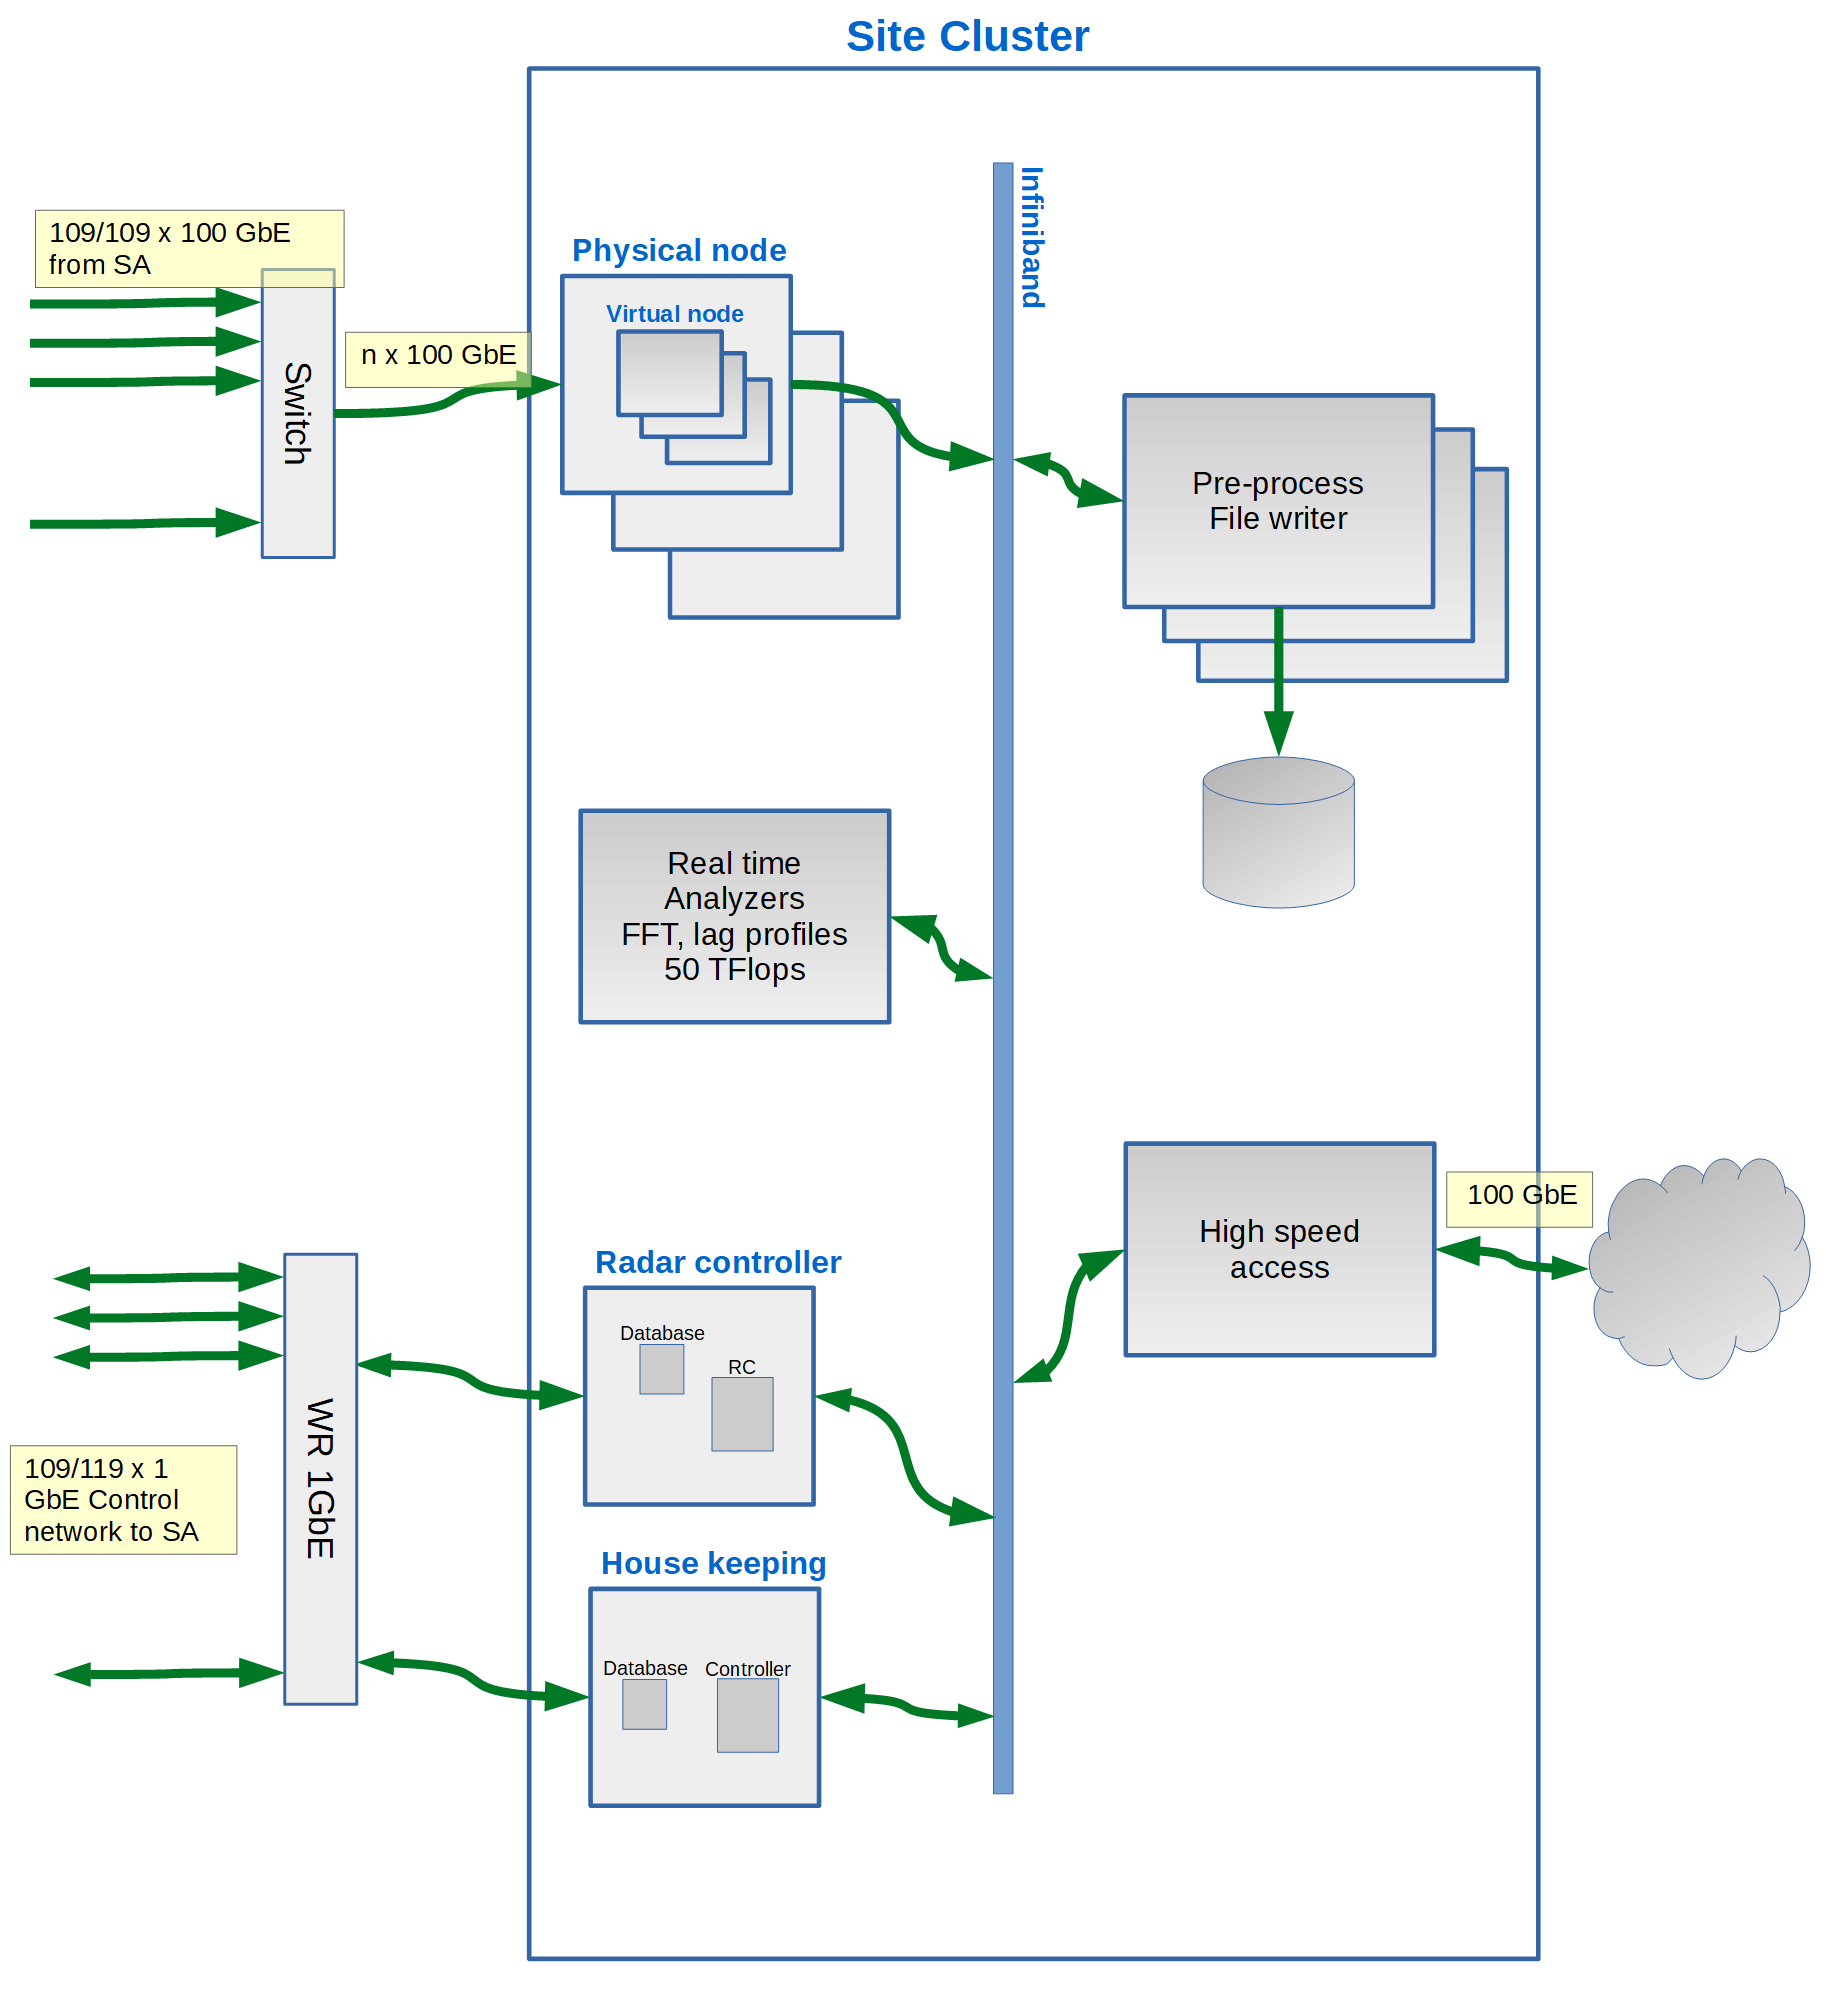
\includegraphics[width=0.8\textwidth]{E3D_dataflow_3aa.png}
\caption{Overview of the site computing hardware including control and analysis hardware. The various site clusters are connected by high-speed network e.g. Infiniband. \label{fig:sitecluster}}
\end{figure}


\subsection{First Stage Receive Unit rates}
\label{ssec:bfrates}

A general description of the {\bf F}irst {\bf S}tage {\bf R}eceiving {\bf U}nit (FSRU) units can be found in~\cite{fsru-tender}. 
Development has started and the final design will be ready by February 2019. 
There will be one FSRU per sub-array having 182 analog channels from 91 antennas. 
After analog-to-digital conversion, signals are delayed and combined to form 10 wide angle beams having two polarizations each.

The original design was to use 100 Gb/s links from each FSRU to the cluster computer, but the possibility to use two 25 Gb/s optical links instead has been studied and proposed to the FSRU supplier.  

One 25 Gb/s link cannot deliver the required data rates of the full \WBW\ bandwidth and 10 beams.  


\subsubsection{Skibotn site:}
\label{sssec:rates:skib}

Table~\ref{tab:skib:rates} gives the total data rate from all sub-array first beam-formers at the Skibotn TX site.
For the \NBW{} ``continuous" operation there will be~2 beams per FSRU, 
each FSRU will transmit 0.6~Gb/s.
The the total data rate from all sub-arrays to the ring buffer in \NBW{} bandwidth will be~76~Gb/s.

For the \WBW{} bandwidth mode, anticipated to run only in a ``burst" mode, there are 1~or~2~beams per~FSRU over all the 119~sub-arrays as, by definition, the radar TX and RX directions are along the same line of site at the TX station.
As the \NBW{} and \WBW{} bandwidths are operated simultaneously, the  total data rate is summed to produce 0.54~Tb/s.
\begin{table}[h]
\centering
\begin{tabular}{rcrlr|r}
{Band-} & {Beams} & {Bits $\times$}    & Rate    & Sub- & {Total rate} \\
{width} & {/FSRU} & {Polarities} & {/FSRU} & arrays & \\ \hline
% \NBW{} & 10 & (16+16)$\times$2 & 3.2 Gb/s & 119 & 0.38~Tb/s \\
% \WBW{} & 1 & (16+16)$\times$2 & 1.9 Gb/s & 109 & 0.21~Tb/s \\
% \WBW{} & 2 & (16+16)$\times$2 & 3.8 Gb/s & 109 & 0.42~Tb/s \\
% \WBW{} & 10 & (16+16)$\times$2 & 19.2 Gb/s & 10 & 0.19~Tb/s
\NBW{} & 2 & (16+16)$\times$2 & 0.6 Gb/s & 119 & 0.08~Tb/s \\
\WBW{} & 2 & (16+16)$\times$2 & 3.8 Gb/s & 119 & 0.46~Tb/s \\
\end{tabular}
\caption{Total data rates expected at the Skibotn TX site. \label{tab:skib:rates}}
\end{table}

\subsubsection{Receive sites}
\label{sssec:rates:rx}

Table~\ref{tab:rx:rates} gives the total data rate from all sub-array first beam-formers at the receive sites.
For \NBW{} bandwidth ``continuous" operation there are~10 beams per FSRU, each FSRU will transmit 3.2~Gb/s for a total rate to the ring buffer of 0.35~Tb/s (350~Gb/s to be compared to 76 Gb/s on the TX site).
For the \WBW{} bandwidth mode, anticipated to run only in a ``burst" mode, 
2~beams will be used per sub-array.
In the \WBW{} bandwidth case, the \WBW{} and \NBW{} rates are summed for a total of 0.76~Tb/s of UDP stream data sent to the ring buffer.
\begin{table}[h]
\centering
\begin{tabular}{rcrll|r}
{Band-} & {Beams} & {Bits $\times$}    & Rate    & Sub- & {Total rate} \\
{width} & {/FSRU} & {Polarities}       & {/FSRU} & arrays & \\ \hline
\NBW{}  & 10 & (16+16)$\times$2 & 3.2~Gb/s & 109 & 0.35~Tb/s \\
% \WBW{} & 10 & (16+16)$\times$2 & 19.2 Gb/s & 109 & 2.1~Tb/s \\
\WBW{} & 2 & (16+16)$\times$2 & 3.84~Gb/s & 109 & 0.41~Tb/s \\
\end{tabular}
\caption{Total data rates expected at the receive sites. \label{tab:rx:rates}}
\end{table}
%% 2 beams for 30 MHz for first five years.

\subsection{Input network}
\label{sec:inputnet}

The input network delivers the 2180 UDP streams through either $2 \times 25$ Gb/s or $1 \times 100$ Gb/s interfaces per \fsru (109 or 119 depending on site) through fiber optic links from each \fsru to the $n$ server nodes that contain the RAM \RB. 
These are the same nodes that perform the second level beam forming: the name \SBF node and \RB node are interchangeable.
There is a choice between connecting the \fsru links directly to ``n" \RB (or \SBF) nodes as shown in Figure~\ref{fig:inputnet-direct} or have a switching fabric in between, as shown in Figure~\ref{fig:network-layer}.
\begin{figure}
\centering
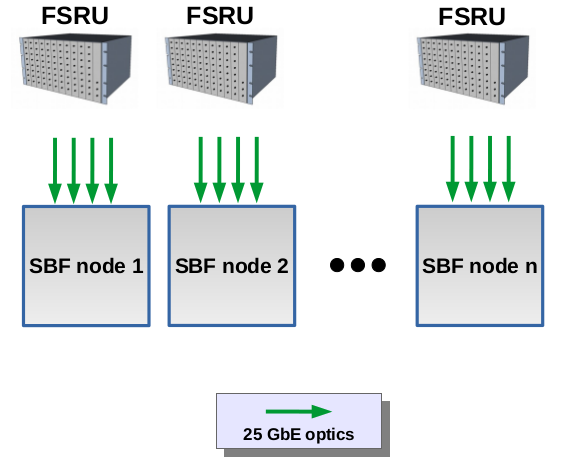
\includegraphics[width=0.4\textwidth]{input_network_7.png}
\caption{Input network that assumes 2x25~Gb/s optical connections from each FSRU directly connected to the second beam former nodes.
\label{fig:inputnet-direct}
}
\end{figure}

%%% CFE: this is a strange sentence. a) is the loss of resolution worse with a switch fabric? b) syntax of the sentence
The advantages of a direct connection of the \fsru links is that the loss of a single component will only result in a fractional loss of $1/n$ of the inputs, which results in lower resolution but still judged to be usable data for $n>10$. 
It also puts constraints on the ``n" \RB nodes since each must provide $238/n$ 25~Gb/s interfaces, in addition to an internal communications fabric between the \RB nodes and a normal interface for exporting data products and system management. 
A quick market survey has put the upper limit on the number of useful 25~Gb/s interfaces per 
2U server at 12 or 13.

A switching fabric (shown in Figure~\ref{fig:network-layer}) allows flexible fail-over through the ability to switch any \fsru to any \RB node, which is helpful from a reliability point of view, as we can assume that server nodes will need scheduled maintenance or will have unscheduled failures.
Recovery from this situation in a fully switched network situation with at least one spare (n+1) \RB node can be done in milliseconds, compared to hours or days if someone has to travel to a remote site. Having a unique destination IP and unique port for each first level beam is also convenient for the software solution.

Switching also means that the \RB nodes only need one 100~Gb/s interface per node for the incoming data, and thus more compact servers are possible.

The downside is the extra cost for switches and that the switch itself will be a single point of failure that can stop a site.

\begin{figure}[ht]
\centering
% 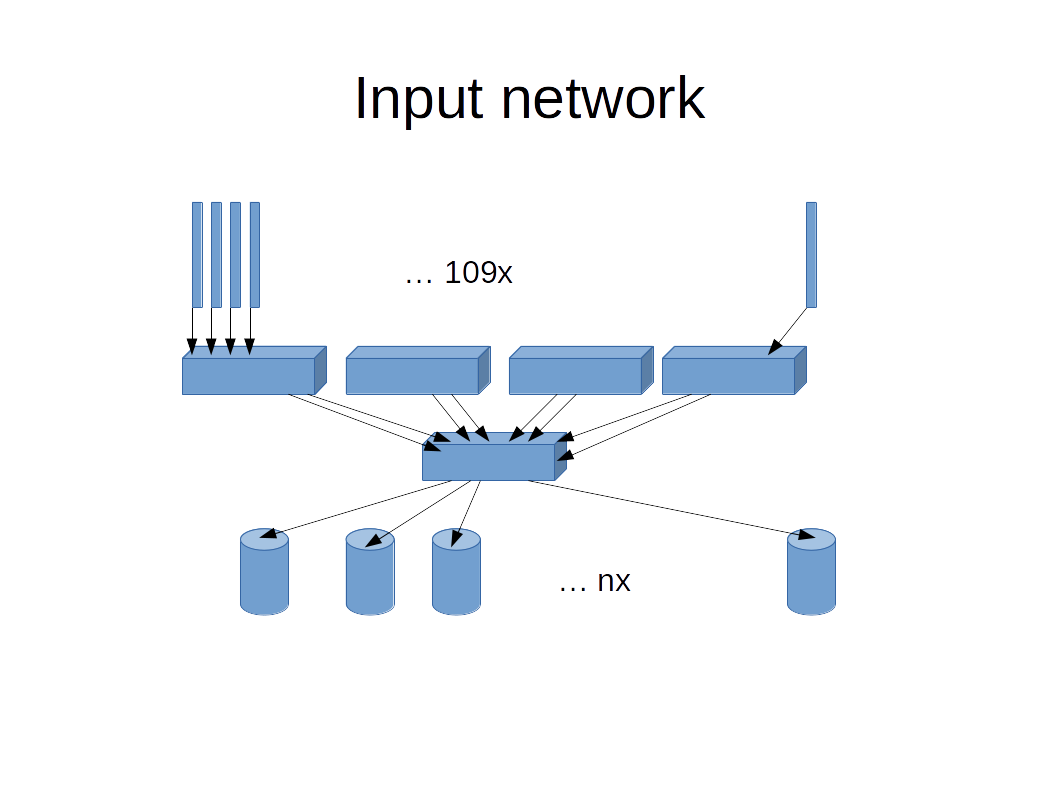
\includegraphics[width=0.9\textwidth]{E3D_inputnetwork.png}
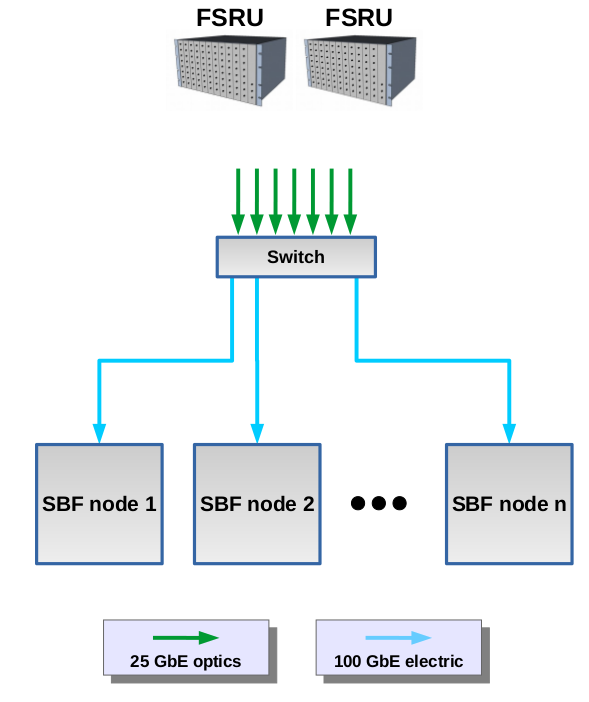
\includegraphics[width=0.4\textwidth]{input_network_8.png}
\caption{Input network candidate that assumes 2x25~Gb/s optical connections from each FSRU to a layer 3 switching infrastructure. A earlier option uses a single 100~Gb/s optical connection to the switching infrastructure. \label{fig:network-layer}
}
\end{figure}


%CFE: commented out repeated discussion
% and also allows fast and flexible fail-over, where any node can take any beam.

%However, a switch is not needed to build the cluster and it will be a single point of failure which can stop all data streams at one site. 
%The number of cluster nodes will be big and one node, in case of failure, will have only small effect on the signal amplitude and resolution.

\subsection{Ring Buffer}
\label{ssec:ring-buffer}

The \RB is a pool of fast-access storage (DRAM, Flash, Phase-Change memory, etc) that is integral to the SBF nodes. 
The beam data packets (b${_s} {^n} {_p}$) from the FSRU are written to the \RB memory.
The \RB size is based on the baseline \NBW{} bandwidth operation and is sized for 
the time that level-1b data can be written to the storage to be processed off-line or written to the disk buffer. 

The minimum \RB should allow 100~s of \NBW{} bandwidth data to be stored, e.g. in order to search for meteors and space debris in the raw data.
An upper limit on the \RB capacity is to store 1200~s of \WBW{} data, which is required to cover a typical scientific rocket launch with F-region (around 250~km) apogee and calculate posterior beams along the trajectory (Nickolay Ivchenko, KTH, Stockholm, private communication). 
If trajectory data could be obtained in near real time (few minutes), this requirement would be relaxed accordingly as the desired beams could then also be formed with a delay on the order of some minutes. 
The following tables give the calculations for the \RB based on an assumption that the \RB must accommodate a minimum of 100~s of real-time \NBW{} level-1a data and up to the maximum of 1200~s.
% Discussion with Nickolay at Eiscat HQ on 5 December. Will ask ESRANGE about the possibility to obtain trajectory coordinates in near real time.
% Rocket trajectories are usually (re)calculated after the flights based on radar or GPS tracking. If so dump data to the SSDs during the flight.

% \subsubsection{Skibotn site}
% \label{sssec:rb:skib}
The buffer calculations for the Skibotn transmitting and receiving site are shown in Table~\ref{tab:skib:rb}.
These calculations assume that in the \NBW\ mode, the site produces only 2~wide-angle beams (along the current and preceding transmission beams).
In the \WBW{} mode, there are additionally 2~beams.
\begin{table}[h]
\centering\begin{tabular}{lrrr|rr|rr}
{Bandwidth} & {Beams/} & {Bits $\times$}    & {Total rate} & Buffer & Buffer & Buffer  \\
            & {FSRU}   & {Polarity$\times$} & (Tb/s)          & \NBW   & size  & \WBW \\
            &          & {Subarrays}        &              & (s) & (TB) & (s) \\ \hline
\NBW{} & 2 & (16+16) & 0.08 &   & \\
      &    &  $\times$2         &                         %  & 100~s   & 0.95~TB   & 14~s  \\
 & 100   & 1.0 & 15  \\
      &    &  $\times$119                           &      & 400   & 3.8    & 56  \\
 \WBW{}    &    &      & 0.46 & 1200  & 11.4 & 169 
\end{tabular}
\caption{Ring buffer calculations and buffer time for \WBW{} bandwidth operation at Skibotn. 
The buffer time for the \WBW{} operations is based on the assumption that there are simultaneously 2~beams each of \NBW\ and \WBW. \label{tab:skib:rb}}
\end{table}

% \subsubsection{Receive sites}
% \label{sssec:rb:rx}
The buffer calculations for the receiving sites are shown in Table~\ref{tab:rx:rbv2}.
These calculations assume that in the \NBW\ mode, the sites produce 10~wide-angle beams.
In the \WBW{} mode, the sites produce 8-wide-angle beams at \NBW\ and 2~wide-angle beams at \WBW.
\iffalse
\begin{table}[h]
\centering\begin{tabular}{lrrr|rr|rr}
{Bandwidth} & {Beams/} & {Bits $\times$}    & {Total rate} & Buffer & Buffer & Buffer \\
            & {FSRU}   & {Polarity$\times$} &   (Tb/s)           & time   & size  & time \\
            &          & {Subarrays}        &              & (\NBW{}) &  (TB) & (\WBW{}) \\ \hline
\NBW{}       & 10       & (16+16)            & 0.35 &   & \\
      &    &  $\times$2         &                          & 100~s   & 4.4  & 51~s  \\
      &    &  $\times$109                           &      & 400~s   & 17.5  & 203~s  \\
 \WBW{} &  2  &    & 0.41 & 1200~s  & 52.5  &  609~s
\end{tabular}
\caption{Ring buffer calculations and buffer time for \WBW{} bandwidth operation at the RX sites. 
The buffer time for the \WBW{} operations is based on the assumption that there are simultaneously 8~beams at \NBW\ and 2~beams at \WBW. \label{tab:rx:rbv2}}
\end{table}
\fi
\begin{table}[h]
\centering\begin{tabular}{lrrr|rr|rr}
{Bandwidth} & {Beams/} & {Bits $\times$}    & {Total rate} & Buffer & Buffer & Buffer \\
            & {FSRU}   & {Polarity$\times$} &   (Tb/s)   & \NBW   & size  & \WBW \\
            &          & {Subarrays}        &              & (s) &  (TB) & (s) \\ \hline
\NBW{}       & 10       & (16+16)           & 0.35 &                               & \\
      &    &  $\times$2         &                          & 100   & 4.4  & 51  \\
      &    &  $\times$109                           &      & 400  & 17.5  & 203  \\
 \WBW{} &  2  &                             & 0.41         & 1200  & 52.5  &  609
\end{tabular}
\caption{Ring buffer calculations and buffer time for \WBW{} bandwidth operation at the RX sites. 
The buffer time for the \WBW{} operations is based on the assumption that there are simultaneously 8~beams at \NBW\ and 2~beams at \WBW. \label{tab:rx:rbv2}}
\end{table}

As can be seen in the above Tables~\ref{tab:skib:rb} and~\ref{tab:rx:rbv2}, the time that data can be written into the \RB when the \WBW\ mode is in operation is roughly an order of magnitude less time at the Skibotn site and half the time at the receive sites.
This is due to the time requirements (min 100~s and max 1200~s) for the \RB in the \NBW\ mode. 
A consequence is that the size (physical) of the \RB on the Skibotn and receive sites will be different.

The \WBW{} bandwidth is mainly for astronomy and plasma line search (including NEIALs~\footnote{Naturally Enhanced Ion-Acoustic Lines, an asymmetry in the scatter spectrum.} with plasma lines). 
The system will be switched to the high \WBW\ rate when NEIALs are detected, and in this case run the FSRUS at \WBW{} for an interval up to about an hour, overwriting the ring buffer in 10~s intervals and storing those with detected NEIALS to disk for offline interferometry.
%% I change this paragraph based on the sentence above...
The time to write level~1 (a or b) data from the \RB memory to the disk buffer must be considered also. 
Writing the level~1a data out to a spinning hard disk buffer will be at least one order of magnitude slower than receiving it from the FSRUs (depending on the storage bandwidth capacity of the site local buffer). % During this time, new data taking at \WBW{} is not possible until the ring buffer has sufficient free space, and if the entire ring buffer is used for \WBW{} data, \NBW{} operation will also need to be paused.

An option for writing level~1a data in burst mode is to use local Solid State Drives (SSDs) i.e. SSDs installed in the \RB nodes. 
SSDs that can handle up to 2-3 Drive Writes Per Day cost much less than RAM, probably adding only 5-10 percent to the \RB costs. 
This means the \WBW{} data could be flushed from the \RB in only 2-4 times as long as it took to receive from the source and enable rapid resumption of \NBW{} operations. 
This is under the assumption that \WBW{} burst mode with raw data dumping would not occur more than 2-3 times per day on a long term average. 
% how about 10-s bursts with post-beam forming on ringbuffer data during following low duty cycle mode?

\subsection{Second beam former rates}
\label{ssec-sbf-rates}

The {\bf S}econd {\bf B}eam {\bf F}ormer (SBF) consists of 
{\bf F}inite {\bf I}mpulse {\bf R}esponse (FIR) filters.
The output of the SBF is 10~narrow angle beams per polarity, with a design possible to scale to 100~narrow angle beams per polarity. 
Each output beam uses data from one wide angle beam on each \fsru so that each narrow angle beam,$B^2_a$, is a summation of data from FIR filters acting on $b^2_{1~a} \ldots b^2_{109~a}$ 
%%% CFE: What does superscript 2 mean? Polarisation channel or level?
\begin{figure}[!h]
\centering
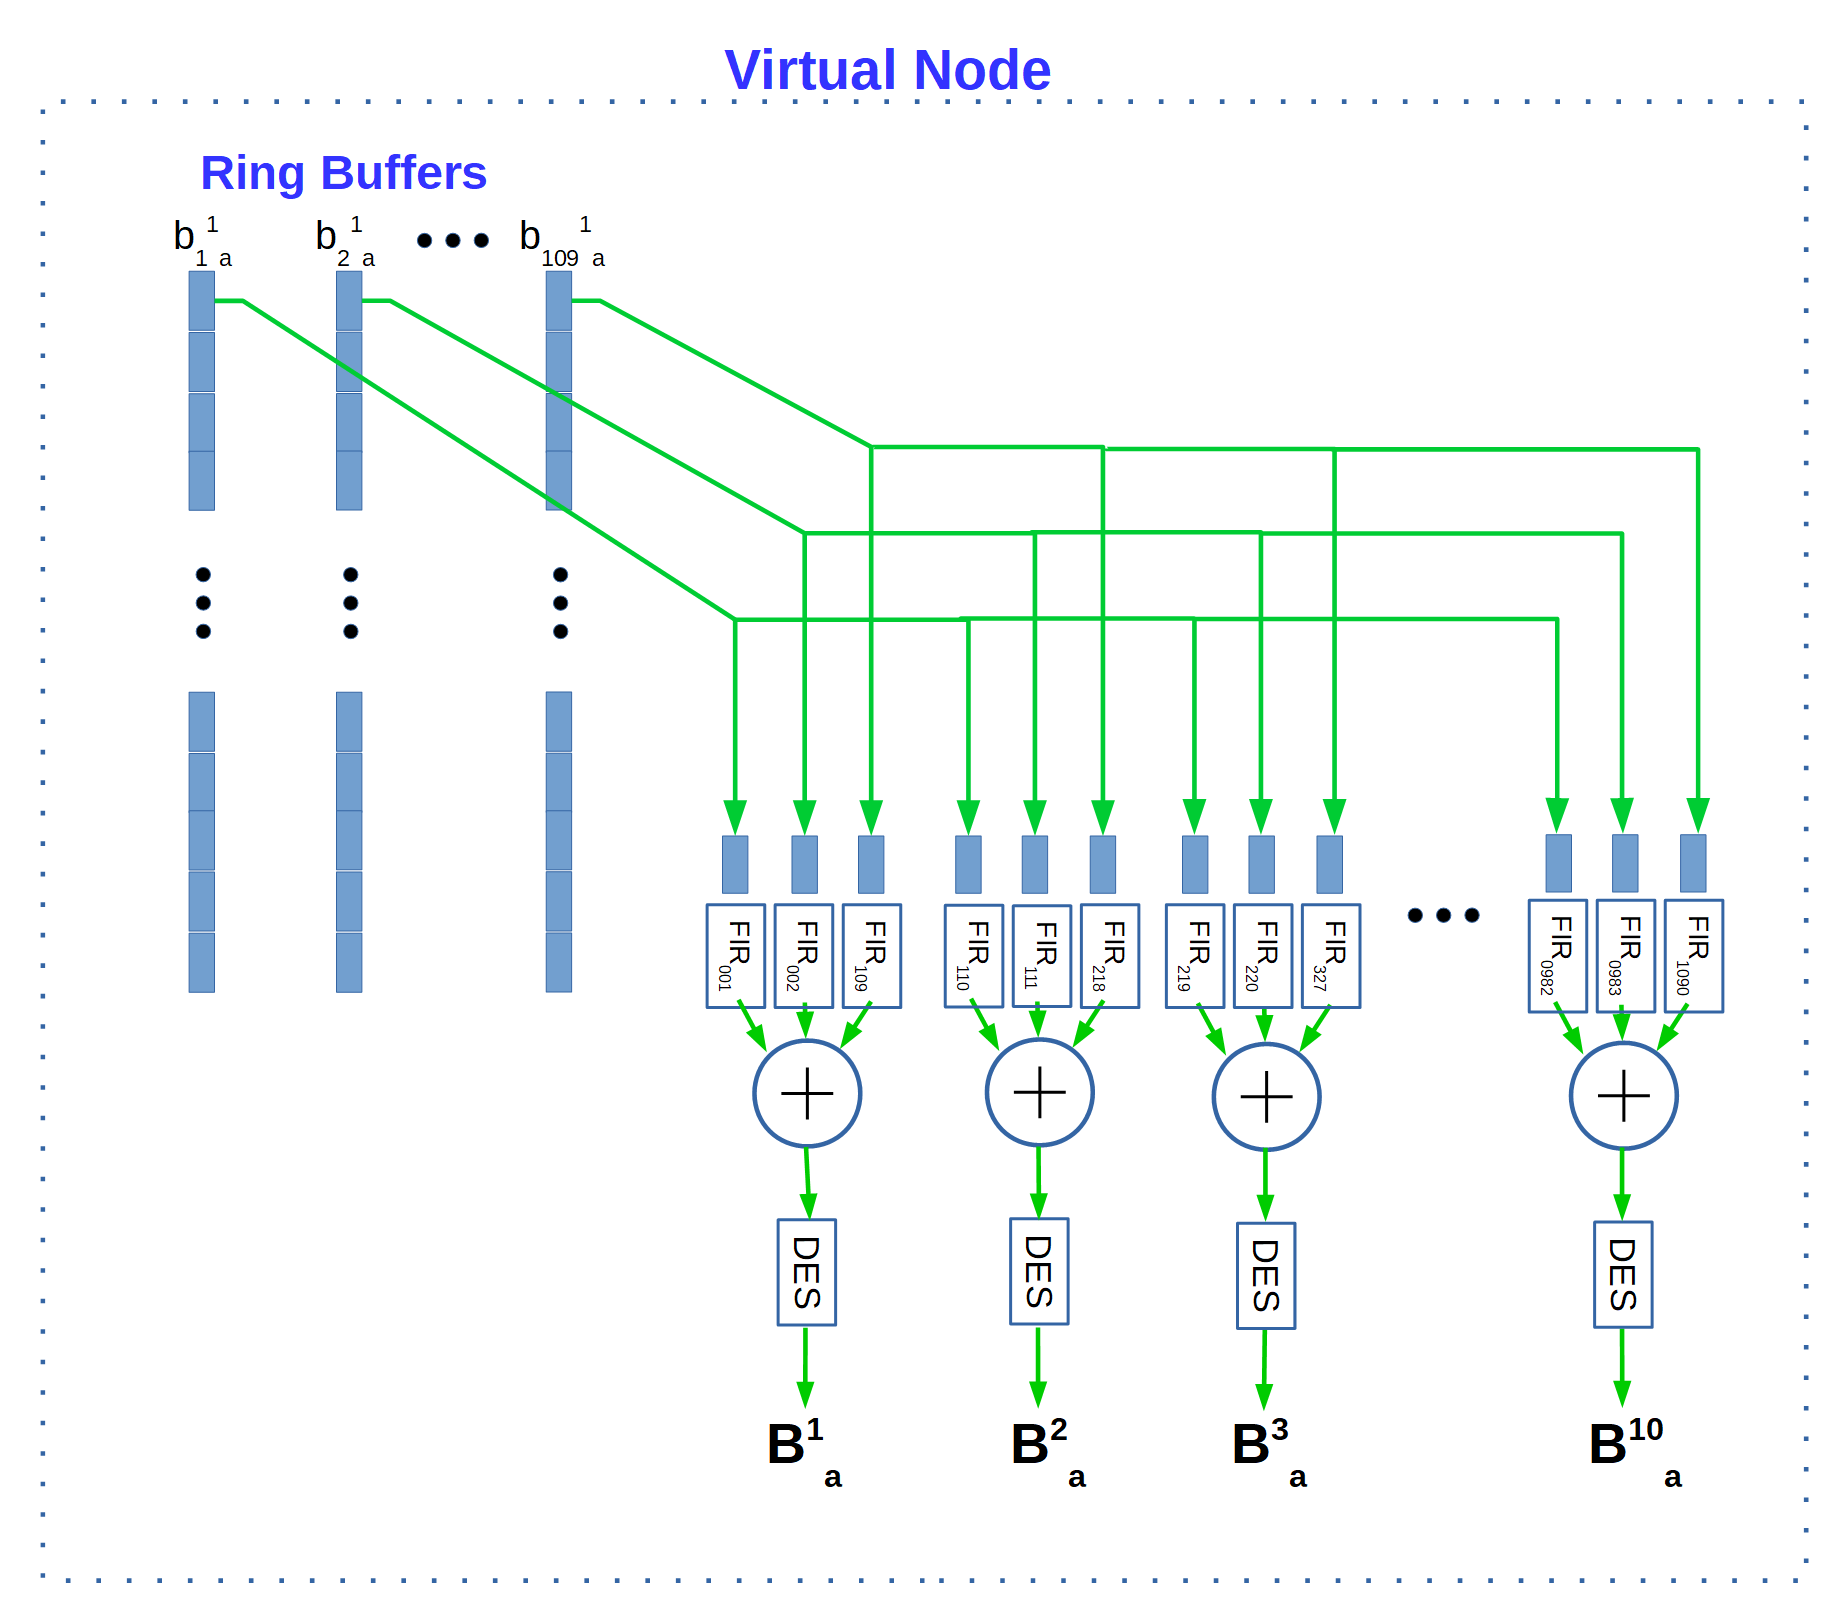
\includegraphics[width=\textwidth]{E3D_dataflow_2aa.png}
\caption{The creation of 10 narrow angle beams (in polarity ``a") through FIRs and summation, showing how each output beam needs input from one beam from each subarray~\label{fig:beams}}
\end{figure}

%% FIXME: Proper reference to Assar's stuff, or copy and paste a bunch?
% CFE: not necessary to repeat
% The beam forming, at the RX sites, that produces 10 narrow angle beams per polarity from each wide angle beam requires 
The beamforming thus requires $109\times 2\times 10\times 10=21800$ FIR filters in total. From the note at~\cite{assars-note} this implies a processing power of 13380~GFLOPS to process \NBW\ data in real time. 
% JW. Fixed the line above.
% CFE removed unnecessary repetitions below
Benchmarks from~\cite{assars-note} has put the performance of modern CPUs at roughly up to 600~GFLOPS per dual CPU node. 
% This leads to a a need for 35-40 nodes at the RX sites in order to beam-form the \NBW\ data in real time.
This leads to a minimum requirement of some 40 2U servers in the\SBF at the RX sites.
The number of SBF nodes required for the CPU part of the beam forming is expected to change downwards as the optimization and testing of the beam forming code proceeds.
At the TX (Skibotn) site, the number of input wide angle beams at \NBW\ is 2 vs 10 which implies a reduction in the required computing capacity by a factor of 5, giving 8 2U nodes.

After the FIR filters the data have to be summed, which aggregates to a large data rate. 
For a naive implementation of just sending all the data for each narrow angle beam to a destination node for summation, a 200~Gb/s network fabric would be needed for the summation alone. 
By summing the values from more than 15 wide angle beams within each node, a 100~Gb/s network will be adequate.

Currently, as explained in~\cite{assars-note} (Section 2.3.1), the summation of the beams within the test servers of the SBF nodes encounters a memory bottleneck that lowers the overall processing speed.
Using the benchmark for the summation within the SBF nodes would imply that the number of SBF nodes would need to increase.
An current estimate from~\cite{assars-note} increases the number of 2U nodes by a factor of 1.5.

A high-performance interconnect such as Infiniband~\cite{infiniband} or Omni-Path~\cite{omnipath} with a focus on parallel computation and low overhead RDMA is suggested to leave as much CPU power as possible in the SBF nodes for the necessary calculations. 
For Infiniband there is also the intriguing possibility of using functionality in the network switch to do the summation inside the switch instead of in the nodes. 
An important design point for this network component is that single switches have 36, 40, or possibly 80 ports. 
But since the cross-node summation only needs to happen within one polarization, splitting the nodes over two switches is fine and more than 72 nodes in total should hopefully not be needed.

\subsection{On-site local disk buffer}

After the narrow angle beams are summed in the \RB nodes, the data streams need to be ordered into files and then shipped off site to a data center for permanent storage. 
In order to handle short interruptions and the occasional inefficient scheduling, a local buffer of at least a few minutes and preferably a few hours is needed.

The total output of the second level beam former is $32+32$ bits $\times$ 200 beams $\times$ 5~MHz = 8 GB/s 
at \NBW{} operations. 
%%%! Tjulin: I get confused easily. Wasn't it 10 narrow beams (2 polarisations) in the previous section?
% JW: Corrected 10 n-a beams per w-a beam
As mentioned in Section~\ref{ssec:ring-buffer} the \RB (or SBF) nodes can be equipped with SSDs.
For example, six 400 GB SSDs in a raid~5 configuration provide 2~TB net usable buffer space, which turns into 250 seconds or $n\times 6$ minutes of effective buffer space in the \NBW{} case, and a sixth of that for \WBW{} (\WBW{} will (can)not be beam formed in real time on the available compute resources though). 
This would also be a fast (2--4~GB/s on each node) target for saving sections of the \RB, where speed of writing is important to free up that part of the \RB for new data.

Using Non-Volatile Memory express (NVMe) for these SSDs might add a bit of cost (list prices are 1.2 times more expensive) but indications are that in a competitive tender the difference is not so big.
Also NVMe reduces CPU usage for I/O and increases total speed.

\subsection{Additional servers for services}
Operations of the experiment and maintenance tasks for the computing requires a highly available database as well as several servers to handle orchestration, software maintenance tasks, file transfer scheduling, etc. %%%! Tjulin: What is a highly available database? What does orchestration mean here?
A system to run highly available databases and virtual machines could echo the one used by the NeIC NT1, and need three physical hosts with local storage.

For maximum commonality, three more nodes with the same specification of the SBF nodes would be appropriate.
As a compromise to reduce the cost, they could be ordered with significantly less RAM (200--300~GB) and only 2 or 4 network interfaces.
%%%! Tjulin: Suggestion "As a compromise to reduce the costs, they could be ordered..."
% JW: changed.
%%%! Tjulin: It feels as this section needs some polishing.
% JW: Agreed... but this subject is almost completely up in % the air still. There's no prototype to even guess the % requirements on hardware. Could put a comment in the conclusions?

\subsection{Output network}

The data produced in the SBF, control updates, as well as general remote management requires connectivity to the datacenter (and directly or indirectly the internet). 
The wide area network connectivity will provide one 
% 100~Gb/s 
100~Gb/s network link.
% or $10 \times 10$~Gb/s.
%HH: 10 -> 100 Gb/s 
This should be connected to one (or several) switches that have enough ports to connect to all the SBF nodes as well as the VM hosts at 10 or 25~Gb/s. 
Such a switch could be a $48 \times 25 + 6 \times 100$ Gb/s switch.

If redundancy here is needed, it could be possible to have two switches in active/passive mode, but this would add both cost and complexity while the expected failure rate of quality networking equipment is generally very low. 
Two switches with any kind of automatic or remote failover capability would also mean two interfaces on every host and in the wide area router. 
% If manual cable movement is needed one might as well just have one spare in the EISCAT offices.
If any manual re-cabling is required in the event of a output network switch failure then ideally there will be a spare unit at the Skibotn TX site and one at the EISCAT headquarters in Kiruna.
The RX sites in Sweden and Finland are reachable by car within 2~hours from Kiruna, Skibotn is 4~hours.
%%%! Tjulin: EISCAT offices on site or EISCAT Headquarters?
% JW: changed text.

\section{On-site software}
\label{sec-onsite-sw}
%%%! Tjulin: The language in this full section seems a bit "Finnish". I think a number of minor edits is needed (add some "the", "a", ...)
% JW: edited HH: Thanks :)
\begin{figure}[!ht]
\centering
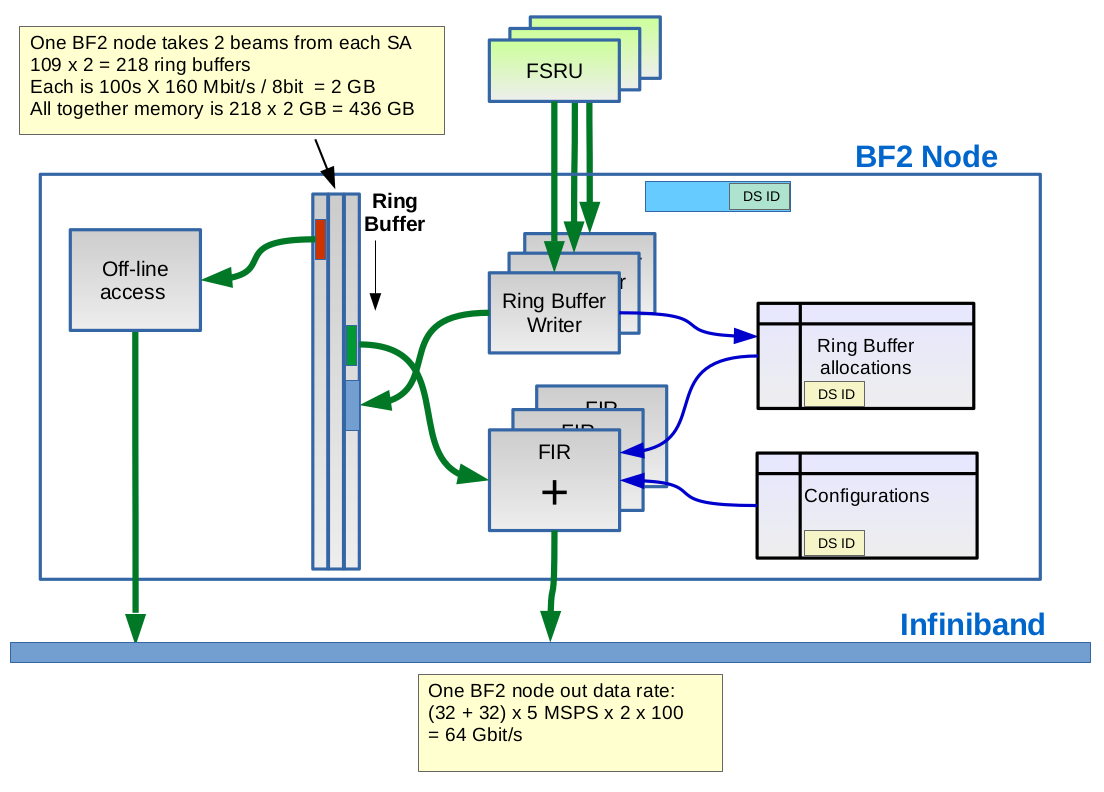
\includegraphics[width=\textwidth]{E3D_dataflow_g_4.png}
\caption{A schematic view of the different software components of the \SBF.}\label{fig:bf2node}
\end{figure}

\subsection{Receiver and \RB process}

A suggested design is to run a process (the \RB process) for each first level wide-angle beam, that listens to a dedicated port and puts all the received data into a \RB in the shared memory of the server node. 
The process reads the data stream index number from the data packet header and updates the \RB database table so that received data can be associated with corresponding data stream.

Once a predefined number of data packets from all \SA{}s have been written to the \RB, the process triggers the \SBF FIR filter process dedicated to this first level beam.

The \RB keeps the data so that in case post-analyzer process finds an interesting event, the corresponding data can be marked as protected and to be downloaded separately. 
This will be done in a database table. 
These \RB areas will not be used for new data until they are released by higher level control (i.e. after the data is downloaded to the local buffer).

\subsection{Second level beam former}

A \SBF process with correct delay and decimation values is implemented when experiment is formed. 
The \SBF process is executed by the \RB when enough data have been received. 
Data stream index and location of the data are given as parameters. 

The \SBF process copies samples to 10 different data flows and runs a FIR filter algorithm through the data. 
The result is 10 different narrow angle beams. 
Early simulations show that one node cannot handle the data rate of all calculated data stream from all \SA{}s, which means that a hierarchical beam forming process will be used. 

Is suggested to be implemented as an MPI~\cite{mpi} program per second level beam produced, that launches on all \RB nodes and one chosen \FW node. 
It would, on each \RB node, continuously read data from the node-local \RB arrays, apply FIR filters on each sample, and then through an MPI\_reduce call do a sum of all the subarray input beams with a target on the \FW node. 
This can also be accelerated by offloading the MPI\_reduce into the switch, as mentioned in Section~\ref{ssec-sbf-rates}.

% * <assar.westman@eiscat.se> 2018-10-21T07:29:40.546Z:
% 
% Is this paragraph starting with "If a simplified.." needed?
% 
% ^ <harri.hellgren@gmail.com> 2018-10-21T14:16:33.312Z:
% 
% No is not. 
%
% ^.

\subsection{File writer and prompt computing}
\label{ssec-fw-prompt}

The \FW process will take the summed narrow-angle beam results from the \SBF and write these to data files
(HDF5-based format suggested) on storage. 
%%% CFE: following sentences have strange syntax.
Instructions for the file sizes, file names and destination folders are in the database written when experiment has been formed. 
The database also includes necessary metadata information which should be written with the actual data.
It is preferred that the HDF5 files will be written to the local SSD buffer on the SBF nodes then transferred to a central location. 
Local storage should be fast so that exceptional events can be downloaded quickly from \RB, so SSD disks are preferred at the site.

The requirements for the \FW processes can be specified by the operating bandwidth (\NBW\ or \WBW) and the level of data reduction within the \SBF. 
The overhead in writing the data to HDF5 files will be negligible as all the experiment-related information is stored in the database and can be added to the HDF5 file system later in the operation center. One narrow angle beam, having \NBW\ bandwidth and two polarizations, is a continuous data stream of 80 MB/s, which is considered very small for any modern SSD disk with write speeds up to 3000 MB/s.  

The \FW processes either run on \SBF nodes or on dedicated nodes, downstream of the \SBF. Dedicated nodes can also be used for summing, decimation, data analyzing and event triggering. 

% repeated ...
%The \FW processes may run on SBF nodes if there is computing and data transfer %capacity available.
%If the SBF nodes are full to capacity then the \FW processes will have to run %on dedicated downstream nodes.


\subsection{Control}
\label{sec:control}

The \ED radar transmissions and receive sites will be controlled by the EROS~\cite{eros} software, used by the current EISCAT radars, re-written for the \ED case.
This will be defined in a future document ``\ED Software Requirement Control Document" that is in preparation.

%% CFE: this can be hard to follow...
The control software will be built around a distributed database. 
Isolated programs can work asynchronously and old EROS programs can be added to the cluster easier.  
The hardware required for the EROS control on each site is not expected to be significant.  %CFE what does this mean?
The computer running EROS must be connected to the 1~Gb/s control network within the site, which also handles timing signals using the \WR synchronization protocol.
This network connects EROS mainly to the Pulse and Steering Control Units (PSCU) and FSRUs located in the Sub-Array Containers under the antenna array. %CFE what does "mainly" mean?

\iffalse
\newpage
\begin{figure}[!ht]
\centering
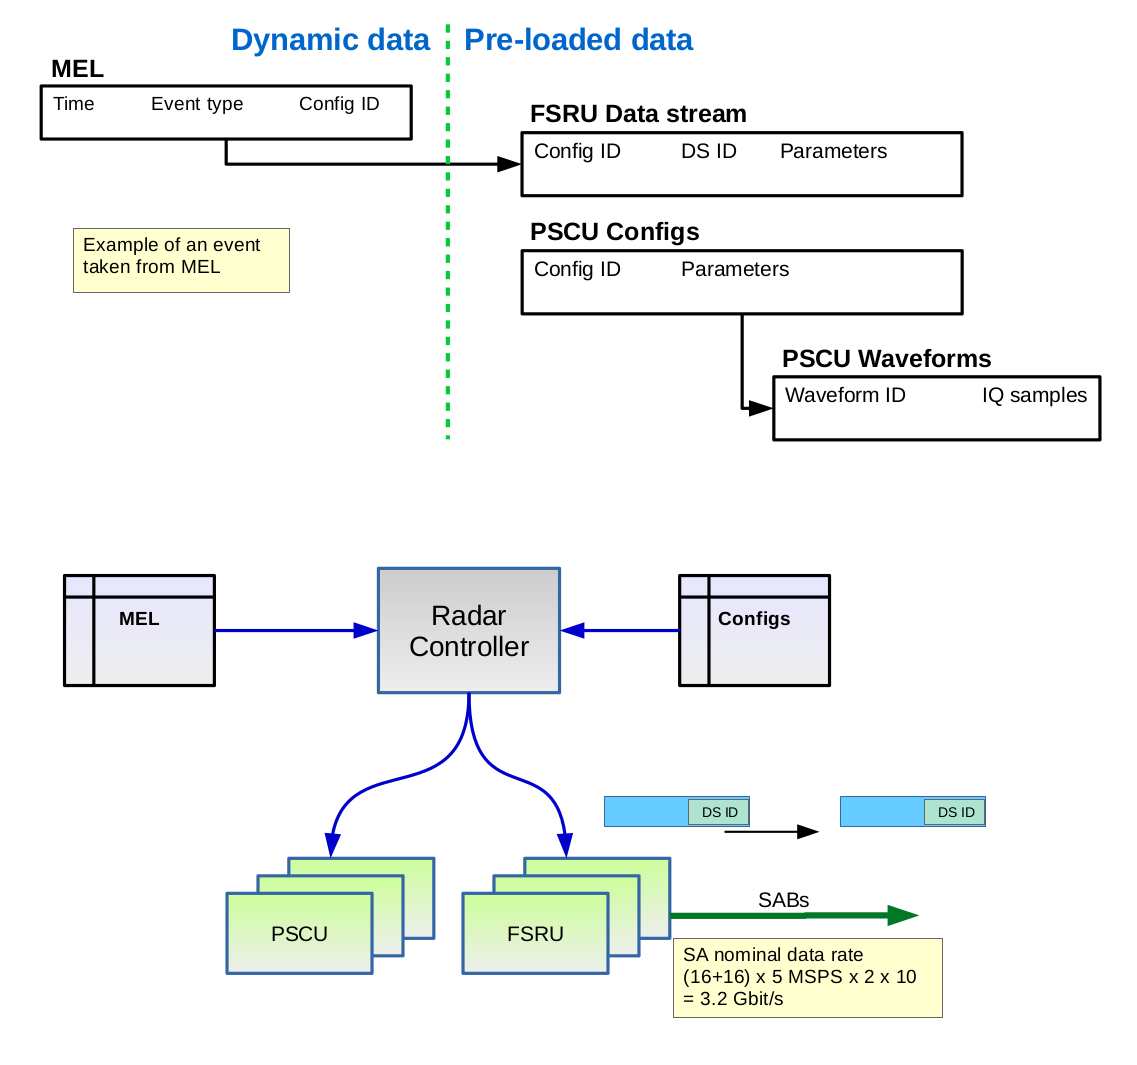
\includegraphics[width=\textwidth]{E3D_dataflow_g_2.png}
\caption{fig 5: A caption for the figure}\label{fig:fsru}
\end{figure}
\fi

\newpage
\bibliography{main}{}
\bibliographystyle{unsrt}

%%%! Tjulin: I corrected the FSRU link in the bib-file.
%%%! Tjulin: In principle, the EROS report link could also be changed into the "official EISCAT" file repository, if it wasn't for the fact that the actual link then would be: https://www.eiscat.se/eiscloud/index.php/s/XH2Y3mQeXat5wdW/download?path=%2FEISCAT_3D%20design%20study%2FWP7%3A%20Distributed%20control%20and%20monitoring&files=EISCAT_3D%20radar%20control%20and%20monitoring%20subsystem%20(March%202009).pdf

\newpage
%\appendix{\large \bf Appendix: Cost estimate}

%%%! Tjulin: Took the liberty to make the appendices included in a more latex-like fashion
% JW: Thanks! Always willing to learn a new latex thing!

\begin{appendices}
\section{Cost estimate}

A cost estimate is shown here based on the text above. 
The costs are based on list prices~\cite{fs-prices} and are made for comparison purposes.
A tender in which sufficient~\footnote{The amount of equipment purchases that trigger discounts varies by supplier and market conditions.} amounts of equipment is being purchased can result in a 30\% reduction in list prices.
Given this observation, standardizing the hardware between the sites and buying under a single tender is the strategy that will deliver the most hardware for money.
%%%! Tjulin: Should define "sufficient" or clean the footnote
% JW: Added more disclaimers.
We assume that the number (and therefore the price) of optical cables and connectors from the FSRUs to the input network and site-local computing (i.e. second beam former) is a constant for all options. 
%%%! Tjulin: What is constant? Price?
% JW number and price.
The output network (Infiniband or other technology after the SBF nodes) is also assumed to be constant, modulo the actual number of SBF nodes.
The cost for a 40-port 200 Gb/s Infiniband switch is 20~k\euro.
Infiniband switches are available with 36, 40, or possibly 80 ports. 

The network switching equipment (between the FSRUs and SBF nodes) has the following prices:
\iffalse
\begin{center}
\begin{tabular}{llc}
{25~\gps}&{100~\gps}   &{Price} \\
{ports} & {ports} & {(k\euro)} \\ \hline
48 & 12 & 30 \\
48 & 6 & 20 \\
48 & 4 & 20 \\ 
0  & 32 & 30 \\
0  & 64 & 80
\end{tabular}
\end{center}
\fi
\begin{center}
\begin{tabular}{llcr}
{25~\gps}&{100~\gps}   &{Price} & {Form}\\
{ports} & {ports} & {(k\euro)} & \\ \hline
48 & 12 & 30 & 1U\\
48 & 6 & 20 & 1U\\
48 & 4 & 20 & 1U \\ 
0  & 32 & 30 &  1U \\
0  & 64 & 80 & 1U
\end{tabular}
\end{center}

The server costs are based on servers in the Kebnekaise cluster at HPC2N in Ume\r{a}
(dual CPU, 2.6~GHz, 14 cores) and 384, 768 or 1532 GB RAM (24$\times$16~GB, 32~GB, 64~GB respectively)\footnote{For performance
all memory channels should have the same population}.
This spec includes 2~TB net SSD on raid-5, enough 25~GbE ports, 100~GbE NIC as a stand-in for Infiniband.
This is the same specification of server as used in the benchmarking in~\cite{assars-note}.
\iffalse
\begin{center}
\begin{tabular}{lc}
{RAM} & {Price} \\
{(TB)} & {(k\euro)} \\ \hline
0.4 & 17 \\
0.8 & 24 \\
1.5 & 40 \\
\end{tabular}
\end{center}
\fi
\begin{center}
\begin{tabular}{lcr}
{RAM} & {Price}  & {Form}\\
{(TB)} & {(k\euro)} & {}\\ \hline
0.2 & 14 & 2U \\
0.4 & 17 & 2U \\
0.8 & 24 & 2U\\
1.5 & 40 & 2U \\
\end{tabular}
\end{center}

The options below, based on the RX sites requirements, correspond to the topologies shown in Figures~\ref{fig:inputnet-direct} and~\ref{fig:network-layer}.
An option based on a variation of Figure~\ref{fig:network-layer} (Fig~\ref{fig:network-layer}$^*$) is also provided where the optical connections from the FSRU input network layer to SBF nodes are 100 Gb/s. 
%%%! Tjulin: Does the asterisked figure exist in this document?
% JW: no ... added a comment to the figure...
The option for server RAM closest to 1~TB RAM is used in each case.
As can be seen in the table, the cost for each option is dominated by the number of \RB nodes.
The main cost driver of the \RB nodes is the amount of RAM.
For example dropping the RAM to 0.4~TB per \RB node gives costs of 716, 788 and 874~k\euro\ respectively.

\newcommand{\sbfN}{40$^*$\xspace}
\iffalse
\begin{center}
\begin{tabular}{llllll}
{Option}&{Optical}   &{Switching} &{SBF}  &{Direct} & {Total} \\
{}      &{Connectors}&{boxes}     &{nodes}&{cables} \\ \hline

Fig~\ref{fig:inputnet-direct}  & $119 \times 2 \times 25$~\gps & n/a & \sbfN & n/a \\
 & 36~k\euro &  & 960~k\euro &  & {\bf 996~k\euro} \\ \hline
Fig~\ref{fig:network-layer} & $119 \times 2 \times 25$~\gps & $2\times$ 48-25 6-100~\gps & \sbfN & \\
   &                               & $1\times$ 48-25 12-100~\gps &     & \\
   & 36~k\euro                     & 70~k\euro                   & {960~k\euro}  &  & 
   {\bf 1066~k\euro} \\ \hline
Fig~\ref{fig:network-layer}$^*$ & $119 \times 2 \times 100$~\gps & $4\times$32-100~\gps & \sbfN & $23 \times 100$~\gps \\
 & 72 k\euro & 120 k\euro & 960~k\euro  & 1.8~k\euro & {\bf 1154~k\euro}
\end{tabular}
\end{center}
\fi
\begin{center}
\begin{tabular}{llllll}
{Option}&{Optical}   &{Switching} &{SBF}  &{Direct} & {Total} \\
{}      &{Connectors}&{boxes}     &{nodes}&{cables} \\ \hline

Fig~\ref{fig:inputnet-direct}  & $119 \times 2 \times 25$~\gps & n/a & \sbfN & n/a & {80U}\\
 & 36~k\euro &  & 960~k\euro &  & {\bf 996~k\euro} \\ \hline
Fig~\ref{fig:network-layer} & $119 \times 2 \times 25$~\gps & $2\times$ 48-25 6-100~\gps & \sbfN & \\
   &                               & $1\times$ 48-25 12-100~\gps &  & & {83U} \\
   & 36~k\euro                     & 70~k\euro                   & {960~k\euro}  &  & 
   {\bf 1066~k\euro} \\ \hline
Fig~\ref{fig:network-layer}$^*$ & $119 \times 2 \times 100$~\gps & $4\times$32-100~\gps & \sbfN & $23 \times 100$~\gps & {84U}\\
 & 72 k\euro & 120 k\euro & 960~k\euro  & 1.8~k\euro & {\bf 1154~k\euro}
\end{tabular}
\end{center}

\newpage
%\appendix{\large \bf Appendix: Future outlook}
%\subsection*{Future hardware outlook}
\section{Future outlook}
\subsection*{Future hardware outlook}

During 2019 new CPU generations from both AMD and Intel will be launched. The AMD processors are expected to bring significant increases in the number and speed of cores, while Intel is expected to bring more modest improvements. Still, a small improvement in the AVX-512 unit could bring big overall performance benefits for our use case.

At the moment AMD has higher main memory bandwidth than Intel server processors, due to four memory channels per processor rather than Intel's three. This difference is foreseen to last at least the next year or two. 

There is also likely that new CPUs will bring PCI Express Generation 4, which is a doubling of the data rate for I/O. This might make it possible to pack more 100~Gb/s network interfaces into a single card or possible to use 200~Gb/s Infiniband. The current roadmaps indicate that AMD will launch CPUs with PICe Gen4 during 2019, and Intel in the middle of 2020.

The biggest cost for the on site computing is the RAM for the ring buffer, which is historically expensive (twice as expensive during 2018 as in 2017). The prices might be going down too.

Newer SSD technologies, either flash or phase change based, might make it possible to build a cheaper \RB\ if they are reliable enough or cheap enough to overprovision sufficiently. Using something else than RAM means moving the data many more times over I/O lanes which probably requires PCIe Gen4 as well as more CPU resources (from HPC2N benchmarks, 2~GB/s disk I/O is enough to saturate a single core, which then is not available for FIR filters).

An interesting possibility for ring buffer storage device is the phase change technology developed by Intel and Micron (Optane\texttrademark). This technology has earlier been used in SATA and NVMe connected storage devices but recently Optane DIMM memory modules has also became available. Optane DIMMs are slower than normal memory modules, but they are able to keep the data permanently in memory. At least in principle, Optane DIMMs could be used in ring buffer instead of normal DIMMs. It is, however, yet unclear what kind of detailed specifications Optane DIMMs have and how competitively they will be priced. In addition, so far Optane DIMMs have been available only for Intel platforms. The use of Optane DIMMs may rule out AMD as a CPU vendor.

The price for 25~Gb/s SFP28 optics modules is likely to drop from today's levels, since this is a very new technology. Rough price parity with 10~Gb/s is expected in a year or two from now, which would cut that cost by almost an order of magnitude.
\end{appendices}
\end{document}
